\documentclass[border=8pt]{standalone}

% Visual reference for the OpenTikZ annotation primitives
% (reference/annotations/annotations.md). One mock pipeline carrying all five.
\usepackage{tikz}
\usetikzlibrary{arrows.meta}
\usetikzlibrary{decorations.pathreplacing}
\usetikzlibrary{positioning, fit, backgrounds, calc}

% --- OpenTikZ palette (light / default, Okabe-Ito) ---
\definecolor{otblue}{HTML}{0072B2}
\definecolor{otorange}{HTML}{E69F00}
\definecolor{otteal}{HTML}{009E73}
\definecolor{otpurple}{HTML}{CC79A7}
\definecolor{otgray}{HTML}{5A5A5A}

\begin{document}
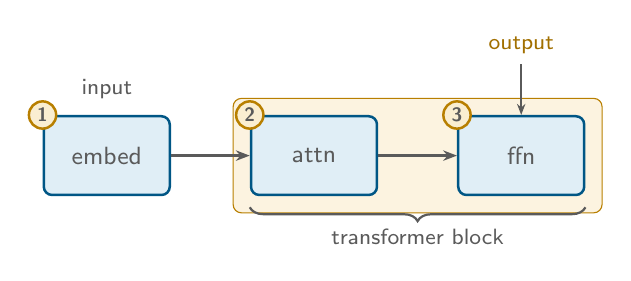
\begin{tikzpicture}[
    line width=0.9pt,
    node distance=10mm,
    block/.style={draw=otblue!75!black, fill=otblue!12, rounded corners=3pt,
                  minimum width=1.6cm, minimum height=1.0cm, text=otgray,
                  font=\sffamily\small},
    lbl/.style={text=otgray, font=\sffamily\footnotesize},
  ]
  % ---- mock 3-stage pipeline ----
  \node[block] (embed) {embed};
  \node[block, right=of embed] (attn) {attn};
  \node[block, right=of attn] (ffn) {ffn};
  \draw[otgray, -{Stealth[length=5pt]}] (embed) -- (attn);
  \draw[otgray, -{Stealth[length=5pt]}] (attn) -- (ffn);

  % (1) text label on a node
  \node[lbl, above=2pt of embed] {input};

  % (2) leader / callout line
  \node[lbl, text=otorange!70!black] (call) at ($(ffn)+(0,1.4)$) {output};
  \draw[otgray, line width=0.7pt, -{Stealth[length=4pt]}]
    (call.south) -- (ffn.north);

  % (3) grouping brace under attn+ffn
  \draw[otgray, line width=0.8pt, decorate,
        decoration={brace, amplitude=5pt, mirror, raise=4pt}]
    (attn.south west) -- (ffn.south east)
    node[midway, below=8pt, lbl, align=center] {transformer block};

  % (4) highlight box around attn+ffn (background layer)
  \begin{scope}[on background layer]
    \node[draw=otorange!80!black, fill=otorange!12, rounded corners=3pt,
          inner sep=6pt, fit=(attn)(ffn)] {};
  \end{scope}

  % (5) step badges
  \foreach \n/\b in {1/embed, 2/attn, 3/ffn}
    \node[circle, draw=otorange!80!black, fill=otorange!18, text=otgray,
          font=\sffamily\scriptsize\bfseries, inner sep=1.3pt]
      at (\b.north west) {\n};
\end{tikzpicture}
\end{document}
